\chapter{月亮在天上}\label{ch:g2:moon-in-the-sky}

有些傍晚，一弯细细的银色月牙挂在屋顶上空；
两周后，一轮圆圆的\omterm{ex:g2:moon-in-the-sky:shapes}{满月}把花园照得一片苍白。它是同一个月亮——
天空中离我们最近的邻居，也是人类唯一踏足过的另一个世界。
现在，让我们好好认识它。

\section{天空中的邻居}

\begin{definition}[月球]\label{def:g2:moon-in-the-sky:moon}
\emph{月球}\index{月球}是一个巨大的灰色岩石球，
绕着地球运行，是我们在太空中忠实的伙伴。它比地球小得多，
而且离我们非常遥远——远到比任何飞机飞得都远，
以至于曾经造访它的宇航员，
花了三天时间才抵达那里。
\end{definition}

\begin{example}[仔细观察]\label{ex:g2:moon-in-the-sky:closely}
用肉眼看月亮，会看到一些浅色的斑块和明亮的区域——
有人甚至能在其中看出一张脸。用双筒望远镜（在\omterm{ex:g2:moon-in-the-sky:shapes}{满月}之夜试试，很有趣）看，
斑块变得清晰，成了平原和一个个圆形的
\emph{环形山}，是很久以前从太空中飞来的岩石
撞到那里后留下的碗状疤痕。\omterm{def:g2:moon-in-the-sky:moon}{月球}永远保留着这些疤痕：它没有风，
也没有雨把它们抹去——事实上，它根本没有\omterm{def:g2:air-around-us:air}{空气}。
没有\omterm{def:g2:air-around-us:air}{空气}，也就意味着一个寂静的世界：在\omterm{def:g2:moon-in-the-sky:moon}{月球}上，
即使大声呼喊，也不会发出任何声音。
\end{example}

\begin{omfigure}
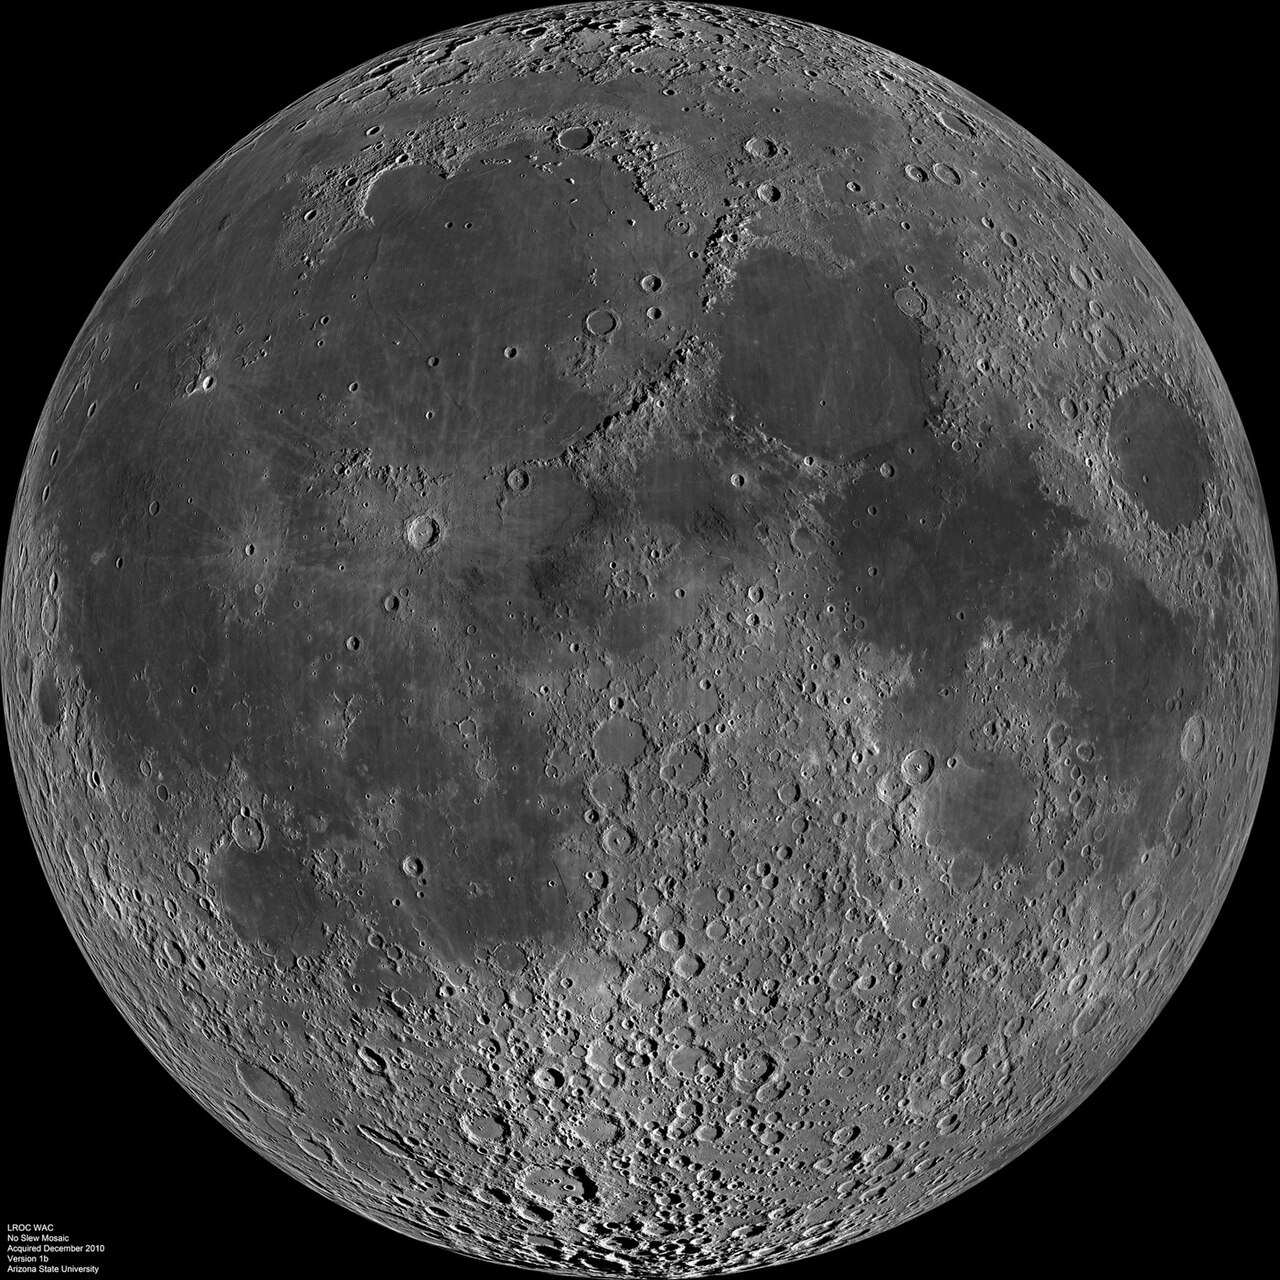
\includegraphics[width=0.44\linewidth]{images/book1/moon-nearside-lro.jpg}

{\small 从轨道上拍摄的\omterm{def:g2:moon-in-the-sky:moon}{月球}正面：
到处是碗状的环形山，还有宽阔的深色平原——却没有\omterm{def:g2:air-around-us:air}{空气}，没有风，也没有声音。
\emph{图片来源：NASA/GSFC/亚利桑那州立大学。}}
\end{omfigure}

\begin{example}[跟着你走的月亮]\label{ex:g2:moon-in-the-sky:follows}
在月光明亮的夜晚沿街走，房屋和树木不断向后掠过，
而月亮似乎始终跟在你的肩头。它其实并没有追着你——
它离我们太远了，走完一整条街，它在你视野中的位置几乎不变，
而近处的房屋却一直在变化。
非常遥远的东西似乎会跟着每一位行人；
月亮做得最好，因为它是“远”的冠军。
\end{example}

\section{反射的光}

\begin{example}[月光是反射的太阳光]\label{ex:g2:moon-in-the-sky:borrowed}
\omterm{def:g2:moon-in-the-sky:moon}{月球}是\omterm{def:g1:light-and-shadows:source}{光源}吗？还记得去年的判断方法吗：它自己会发光吗？
它不会——\omterm{def:g2:moon-in-the-sky:moon}{月球}是一块暗色的岩石球，就像天上的一块大石头。
我们所说的月光，其实是太阳光
被这块岩石\emph{反射}回来，射向我们，
好比一面白墙照亮房间，而墙本身并不是灯。
太阳照亮了\omterm{def:g2:moon-in-the-sky:moon}{月球}的一侧，
我们看到的，是这明亮一侧中朝向我们的那一部分。
\end{example}

\begin{omfigure}
\begin{tikzpicture}[scale=0.85]
  \fill[omThm] (0.7,1.5) circle (0.45);
  \foreach \a in {0,30,...,330} {
    \draw[omThm] (0.7,1.5) ++(\a:0.62) -- ++(\a:0.26);
  }
  \node[below, font=\small] at (0.7,0.8) {太阳};
  \draw[thick] (6.8,1.5) circle (1.1);
  \begin{scope}
    \clip (6.8,1.5) circle (1.1);
    \fill[omExo, opacity=0.5] (6.8,0.3) rectangle (8.1,2.7);
  \end{scope}
  \node[below, font=\small] at (6.8,0.1)
    {向太阳的一面亮，背面暗};
\end{tikzpicture}

{\small 太阳照亮\omterm{def:g2:moon-in-the-sky:moon}{月球}的一半，始终是面向太阳的那一半。
另一半则处于它自己的黑夜之中。}
\end{omfigure}

\begin{remark}[白天的月亮]\label{rem:g2:moon-in-the-sky:daytime}
很多人以为月亮是夜晚的“专属”——
但在一些下午抬头看看，它就挂在那里，像蓝天里的一个淡淡幽灵！
\omterm{def:g2:moon-in-the-sky:moon}{月球}按照自己的节奏绕着地球运行，
并不在乎此时是我们的白天还是夜晚。
只不过白天太阳的光芒洒满天空，月亮显得没那么醒目罢了。
\end{remark}

\section{月亮的形状在变化}

\begin{example}[月亮的形状变化]\label{ex:g2:moon-in-the-sky:shapes}
连续观察许多个夜晚，你会发现月亮的形状在变化：
先是一弯细细的\emph{蛾眉月}\index{蛾眉月}，像一片指甲的碎屑，
然后是半圆，接着是饱满、几乎圆的形状，
最后成为\emph{满月}\index{满月}的完美圆盘——然后再逐渐变回去，
变成朝向另一边的\omterm{ex:g2:moon-in-the-sky:shapes}{蛾眉月}，直到一两个夜晚，月亮似乎完全消失不见。
整个变化过程大约持续一个月，
然后循环重复，像昼夜交替一样准时可靠。
\end{example}

\begin{omfigure}
\begin{tikzpicture}[scale=0.85]
  % dark disc for every station, lit part painted over it
  \foreach \x in {0,2.2,4.4,6.6,8.8} {
    \fill[omExo!75] (\x,0) circle (0.8);
  }
  % crescent: lit right edge only
  \begin{scope}
    \clip (2.2,0) circle (0.8);
    \fill[yellow!30] (2.2,-0.85) rectangle (3.05,0.85);
    \fill[omExo!75] (2.2,0) ellipse (0.5 and 0.8);
  \end{scope}
  % half: lit right half
  \begin{scope}
    \clip (4.4,0) circle (0.8);
    \fill[yellow!30] (4.4,-0.85) rectangle (5.25,0.85);
  \end{scope}
  % almost full: dark left sliver only
  \begin{scope}
    \clip (6.6,0) circle (0.8);
    \fill[yellow!30] (6.6,0) circle (0.8);
    \fill[omExo!75] (5.75,-0.85) rectangle (6.6,0.85);
    \fill[yellow!30] (6.6,0) ellipse (0.5 and 0.8);
  \end{scope}
  % full: all lit
  \fill[yellow!30] (8.8,0) circle (0.8);
  \foreach \x in {0,2.2,4.4,6.6,8.8} {
    \draw[thick] (\x,0) circle (0.8);
  }
  \node[below, font=\small] at (0,-1.05) {新月：不可见};
  \node[below, font=\small] at (2.2,-1.05) {蛾眉月};
  \node[below, font=\small] at (4.4,-1.05) {半月};
  \node[below, font=\small] at (6.6,-1.05) {凸月};
  \node[below, font=\small] at (8.8,-1.05) {满月};
\end{tikzpicture}

{\small 两周的\omterm{def:g2:moon-in-the-sky:moon}{月球}观测：被照亮的部分一夜夜变化，
从无到满盘，然后又缩回去。}
\end{omfigure}

\begin{omfigure}
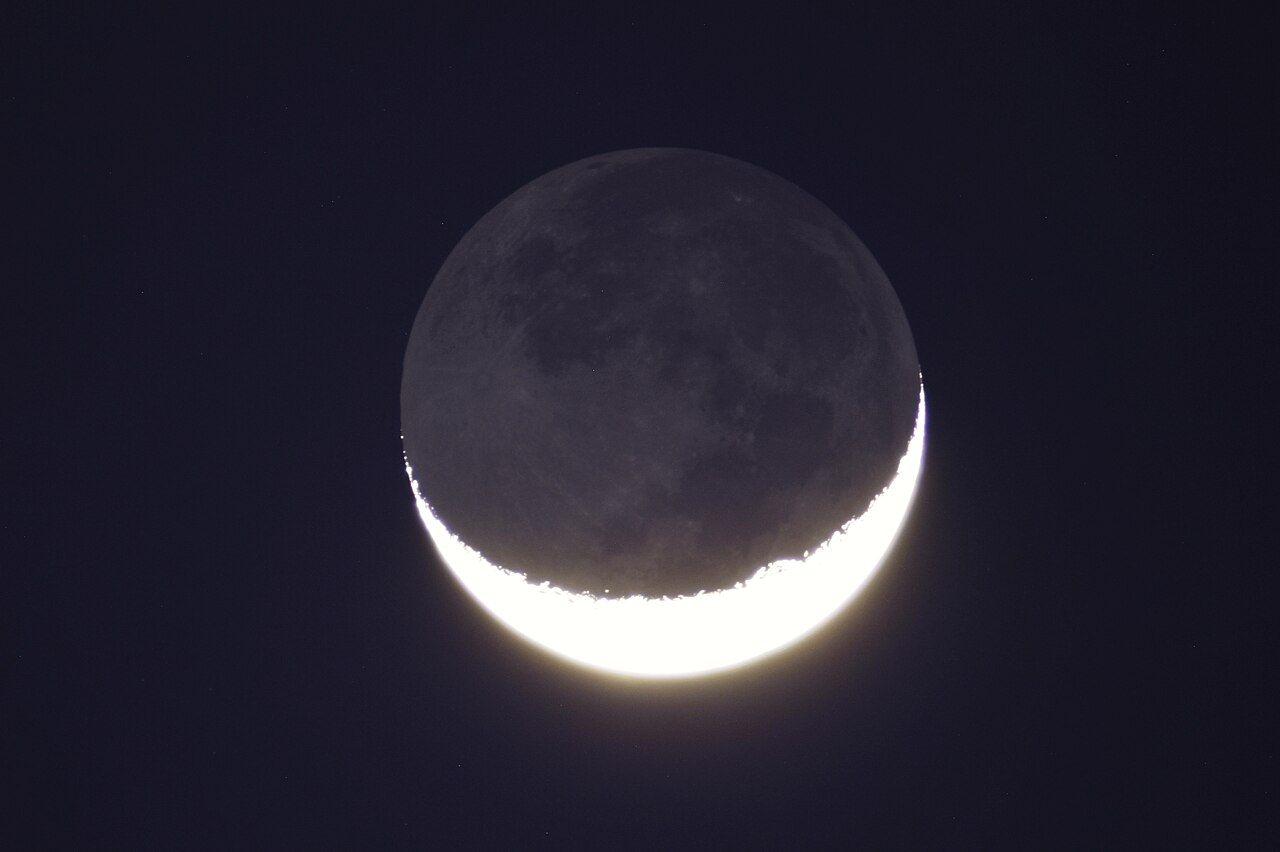
\includegraphics[width=0.42\linewidth]{images/book1/moon-crescent.jpg}\quad
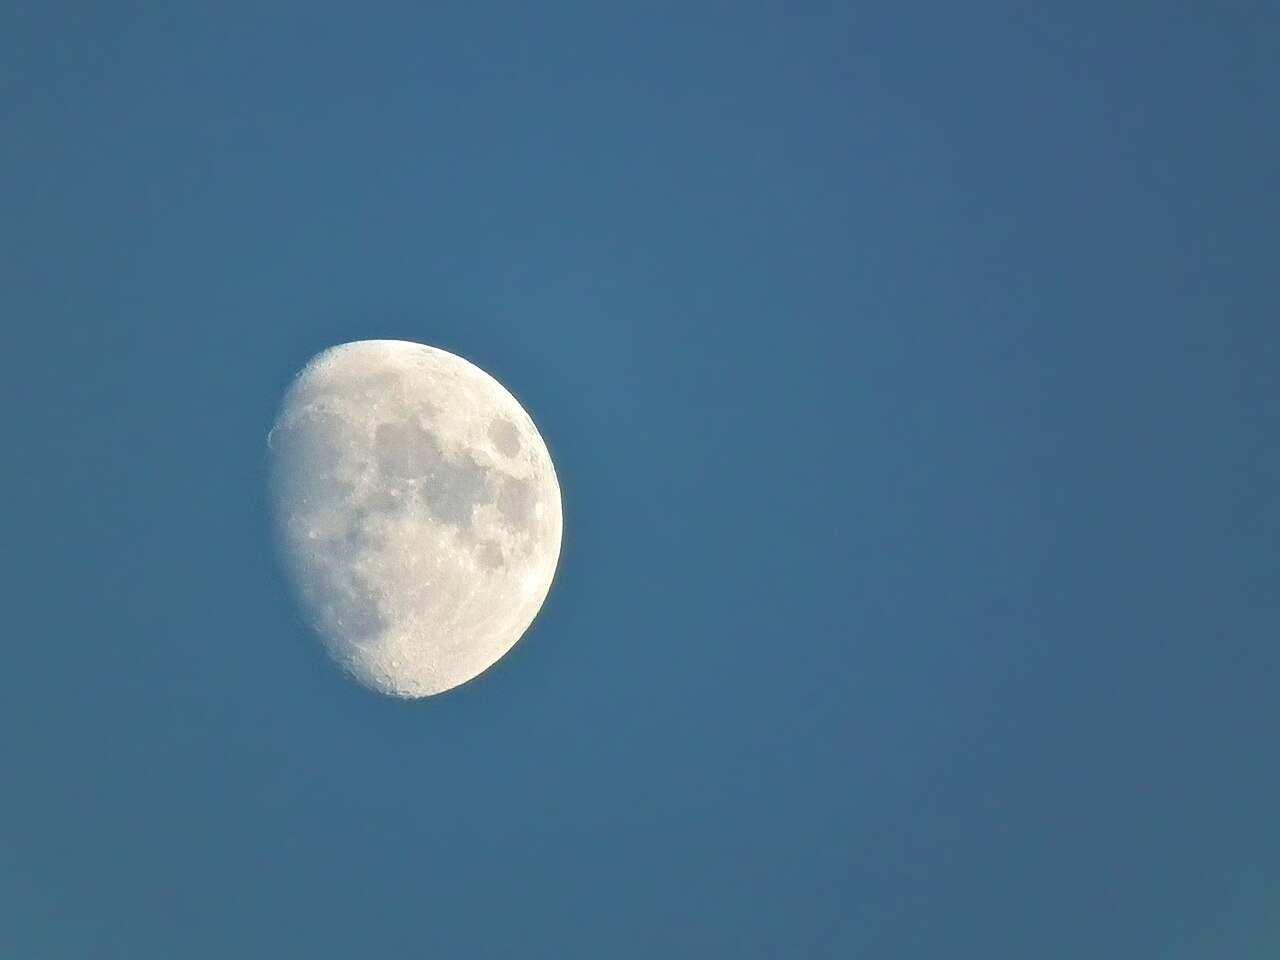
\includegraphics[width=0.42\linewidth]{images/book1/moon-gibbous.jpg}

{\small 真实的月相：左图是一弯细细的\omterm{ex:g2:moon-in-the-sky:shapes}{蛾眉月}（仔细看：圆盘的
暗部也隐隐发光）；右图是白天天空中的近\omterm{ex:g2:moon-in-the-sky:shapes}{满月}。
\emph{照片：G.~Donatiello，CC0；
Cbaile19，CC0。}}
\end{omfigure}

\begin{method}[记录月亮日记]\label{met:g2:moon-in-the-sky:diary}
\begin{enumerate}
  \item 每个晴朗的傍晚，大约在同一时刻，
        找一找月亮；
  \item 在一个小小的日历方格里画出你看到的形状，
        画一个圆，并涂暗部；
  \item 如果云把月亮遮住了，就写下“有云”，然后继续记录；
  \item 两周后，把你的画按顺序排成一排。
\end{enumerate}
你自己的画会显示月相在变化，
每晚都变一点。\emph{为什么}月亮会这样变化，是
一个有趣的谜题——它将在本课程的后面某一年得到正式解答，
而你的日记正是证明的第一步。
\end{method}

\section{练习}

\begin{exercise}[$\star$]\label{exo:g2:moon-in-the-sky:1}
\omterm{def:g2:moon-in-the-sky:moon}{月球}比地球大还是小？它比
云更近还是更远？人们怎么知道能够造访\omterm{def:g2:moon-in-the-sky:moon}{月球}？
\end{exercise}

\begin{exercise}[$\star$]\label{exo:g2:moon-in-the-sky:2}
\omterm{def:g2:moon-in-the-sky:moon}{月球}上那些圆碗状的痕迹叫什么，
它们是由什么造成的？经过这么久为什么仍然存在？
\end{exercise}

\begin{exercise}[$\star$]\label{exo:g2:moon-in-the-sky:3}
\omterm{def:g2:moon-in-the-sky:moon}{月球}是像灯一样的\omterm{def:g1:light-and-shadows:source}{光源}，还是像白墙一样的
光接收体？月光究竟来自哪里？
\end{exercise}

\begin{exercise}[$\star$]\label{exo:g2:moon-in-the-sky:4}
太阳照亮的是\omterm{def:g2:moon-in-the-sky:moon}{月球}的哪一半：总是面向太阳的那一半，
总是同一半，还是随机的一半？
\end{exercise}

\begin{exercise}[$\star$]\label{exo:g2:moon-in-the-sky:5}
\omterm{def:g2:moon-in-the-sky:moon}{月球}能在白天被看见吗？
如果朋友说不能，什么能让他信服？
\end{exercise}

\begin{exercise}[$\star$]\label{exo:g2:moon-in-the-sky:6}
按顺序说出\omterm{def:g2:moon-in-the-sky:moon}{月球}的各种形状，从细细的指甲月开始，
到圆圆的灯笼月结束。大约要多长时间，
整个变化过程才会重复？
\end{exercise}

\begin{exercise}[$\star$]\label{exo:g2:moon-in-the-sky:7}
\omterm{def:g2:moon-in-the-sky:moon}{月球}上没有\omterm{def:g2:air-around-us:air}{空气}。那里的喊声会怎样？
那风筝又会怎样？
\end{exercise}

\begin{exercise}[$\star$]\label{exo:g2:moon-in-the-sky:8}
今晚就开始\cref{met:g2:moon-in-the-sky:diary}中的月亮日记。
每晚必须保持哪两件事不变，
才能让日记公平可比？
\end{exercise}

\begin{exercise}[$\star\star$]\label{exo:g2:moon-in-the-sky:9}
“月亮一路跟着我们的车回家！”小罗莎说。
向她解释，借助
\cref{ex:g2:moon-in-the-sky:follows}中的街道行走例子，为什么非常远的东西看起来会跟着走，
而近处的东西却会向后滑过。
\end{exercise}

\begin{exercise}[$\star\star$]\label{exo:g2:moon-in-the-sky:10}
在\omterm{ex:g2:moon-in-the-sky:shapes}{蛾眉月}的夜晚仔细观察：有时\omterm{def:g2:moon-in-the-sky:moon}{月球}的\emph{暗}部会非常微弱地发光，
因此整个圆几乎只能被猜出来。
太阳并不照亮那一部分，但附近有别的东西在发光。
那么，是什么巨大、明亮、被阳光照耀的球体，
在照亮\omterm{def:g2:moon-in-the-sky:moon}{月球}的暗面，就像\omterm{def:g2:moon-in-the-sky:moon}{月球}照亮我们的夜晚一样？
（提示：你正站在它上面。）
\end{exercise}
